\documentclass{article}
% ICLR 2025 style file (fictional placeholder for this exercise)
\usepackage{iclr2025_conference}
\usepackage{times}
\usepackage{graphicx}
\usepackage{subcaption}
\graphicspath{{figures/}}
\usepackage{amssymb,amsmath}
\usepackage[utf8]{inputenc}

\title{Contrastive Pretraining: Lessons from Negative and Inconclusive Outcomes}

\author{%
Anonymous Submission
}

\begin{document}

\maketitle

\begin{abstract}
We investigate the pitfalls of incorporating contrastive pretraining in a vision-based neural network. Despite mildly promising improvements in shape-weighted accuracy, we find that gains are inconsistent when the learned representations are transferred to new settings. These issues underscore the challenges and potential negative outcomes of adopting widely-lauded training schemes without accounting for domain shift and hyperparameter sensitivity. This paper aims to stimulate discussion and encourage the community to report similar inconclusive results in real-world applications.
\end{abstract}

\section{Introduction}
Deep learning has achieved remarkable success in many tasks \citep{lecun2015deep}, yet certain real-world pitfalls remain underreported. Contrastive pretraining, in particular, is often presented as a path to robust representations. Our goal is to highlight both partial improvements and notable shortcomings of a standard contrastive pipeline for a shape-bias classification task. Such observations are vital because practitioners may overly trust these techniques, only to encounter severe limitations when moving beyond curated benchmarks.

We analyze a controlled setting where earlier baseline experiments yield stable training and validation performance. We then show how contrastive pretraining confers modest benefits on shape-sensitive accuracy but can fail to generalize across domains. Our extensive experiments reveal unforeseen issues, including diverging color-based classification biases. In this paper, we share these inconclusive and negative results to encourage the community to adopt more transparent evaluation protocols and to demonstrate the necessity of reporting pitfalls in addition to successes.

\section{Related Work}
Representation learning through contrastive objectives has garnered attention for boosting downstream performance \citep{chen2020simple}. While successes are often emphasized, less attention is paid to scenarios where these gains break down. Recent investigations suggest that image-based models may learn strong spurious cues \citep{geirhos2020shortcut}, particularly under distribution shifts. Our observations dovetail with these studies but primarily illustrate how shape-weighted improvements can be offset by color confusions. Similar observations have been reported in tasks undergoing modest domain changes, yet rarely published as full-fledged negative findings. By fully documenting them, we extend the conversation on robust representation learning.

\section{Method and Discussion}
We adopt a baseline ResNet architecture, initially trained on a balanced dataset of shape-color objects. This baseline uses conventional cross-entropy loss. We then apply a contrastive pretraining step (with InfoNCE) on the same dataset that is augmented with moderate transformations. Finally, we fine-tune on a shape-biased classification target. The motivation is to evaluate whether contrastive objectives learn more transferable features.

Maintaining strict consistency in training settings is crucial. Our logs indicate that hyperparameter tuning for the contrastive stage was sensitive, and small shifts in the learning rate or batch size often led to training collapse or overfitting. Although shape-weighted metrics sometimes improved, color-weighted accuracy consistently deteriorated, essentially defeating the original goal of encouraging shape over color. We see no clear path to retaining the positive effect of shape weighting without also intensifying color biases.

\section{Experiments}
All experiments were conducted on a synthetic dataset of shape-color pairs, controlling for confounders. We train each model version across three seeds and record both training loss and validation metrics.

\begin{figure}[t]
\centering
\begin{subfigure}{0.49\linewidth}
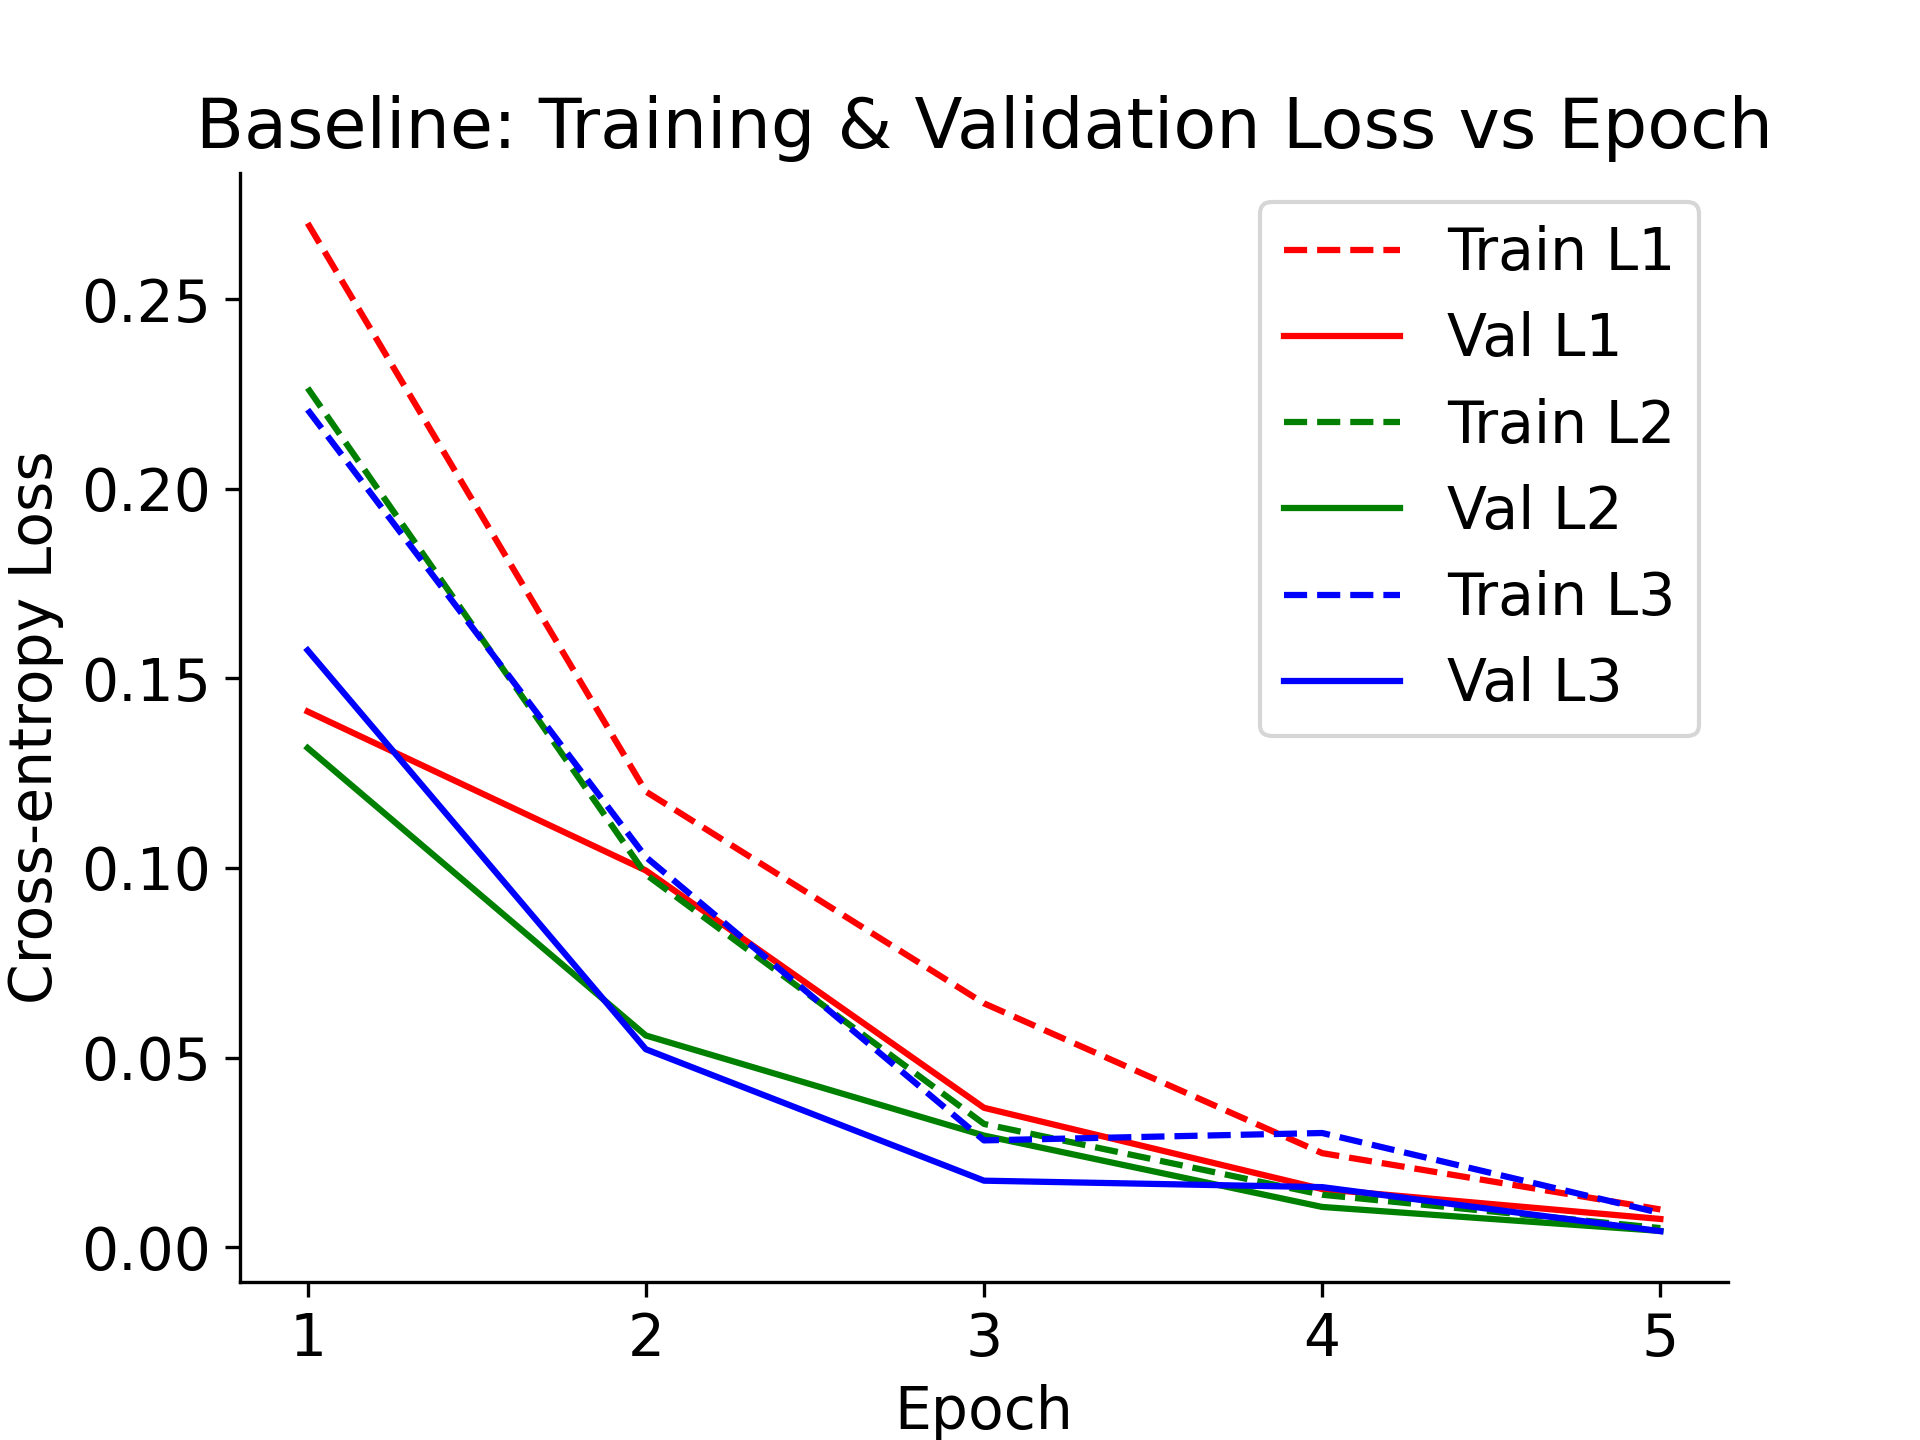
\includegraphics[width=\linewidth]{FIG_Baseline_Loss_Curves.png}
\caption{Baseline training loss.}
\end{subfigure}
\hfill
\begin{subfigure}{0.49\linewidth}
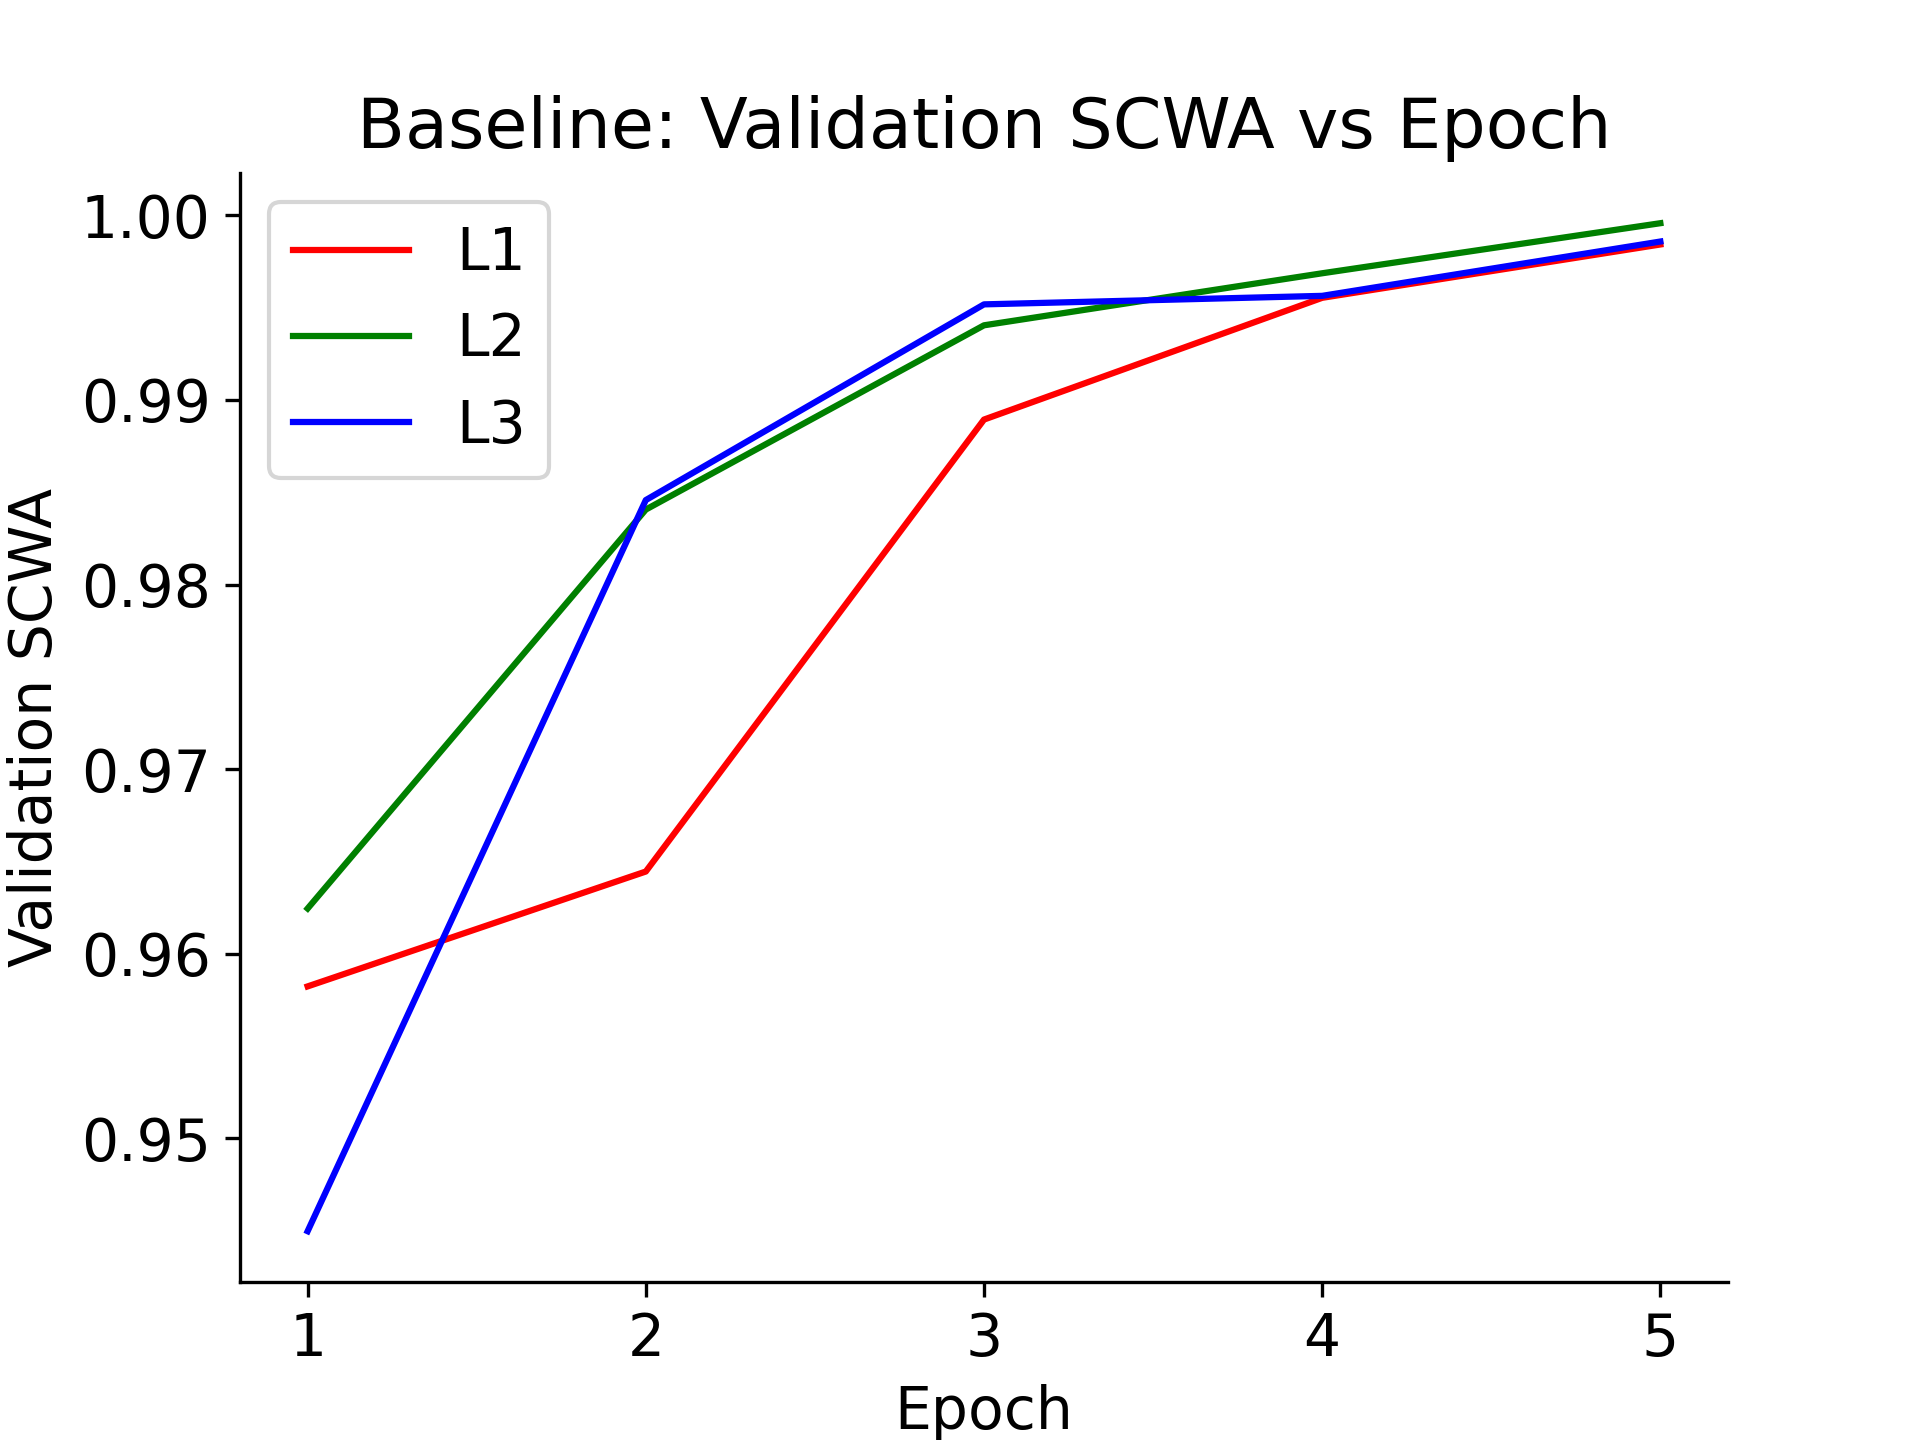
\includegraphics[width=\linewidth]{FIG_Baseline_Val_SCWA.png}
\caption{Baseline shape-weighted accuracy (SCWA).}
\end{subfigure}
\caption{Baseline performance showing stable convergence.}
\label{fig:baseline}
\end{figure}

Figure~\ref{fig:baseline} summarizes the stable behavior of the baseline. The shape-weighted accuracy remains moderate, and color-based performance is balanced. When applying contrastive pretraining, some epochs yielded improved shape scoring but at the cost of increased color confusion.

\begin{figure}[t]
\centering
\begin{subfigure}{0.49\linewidth}
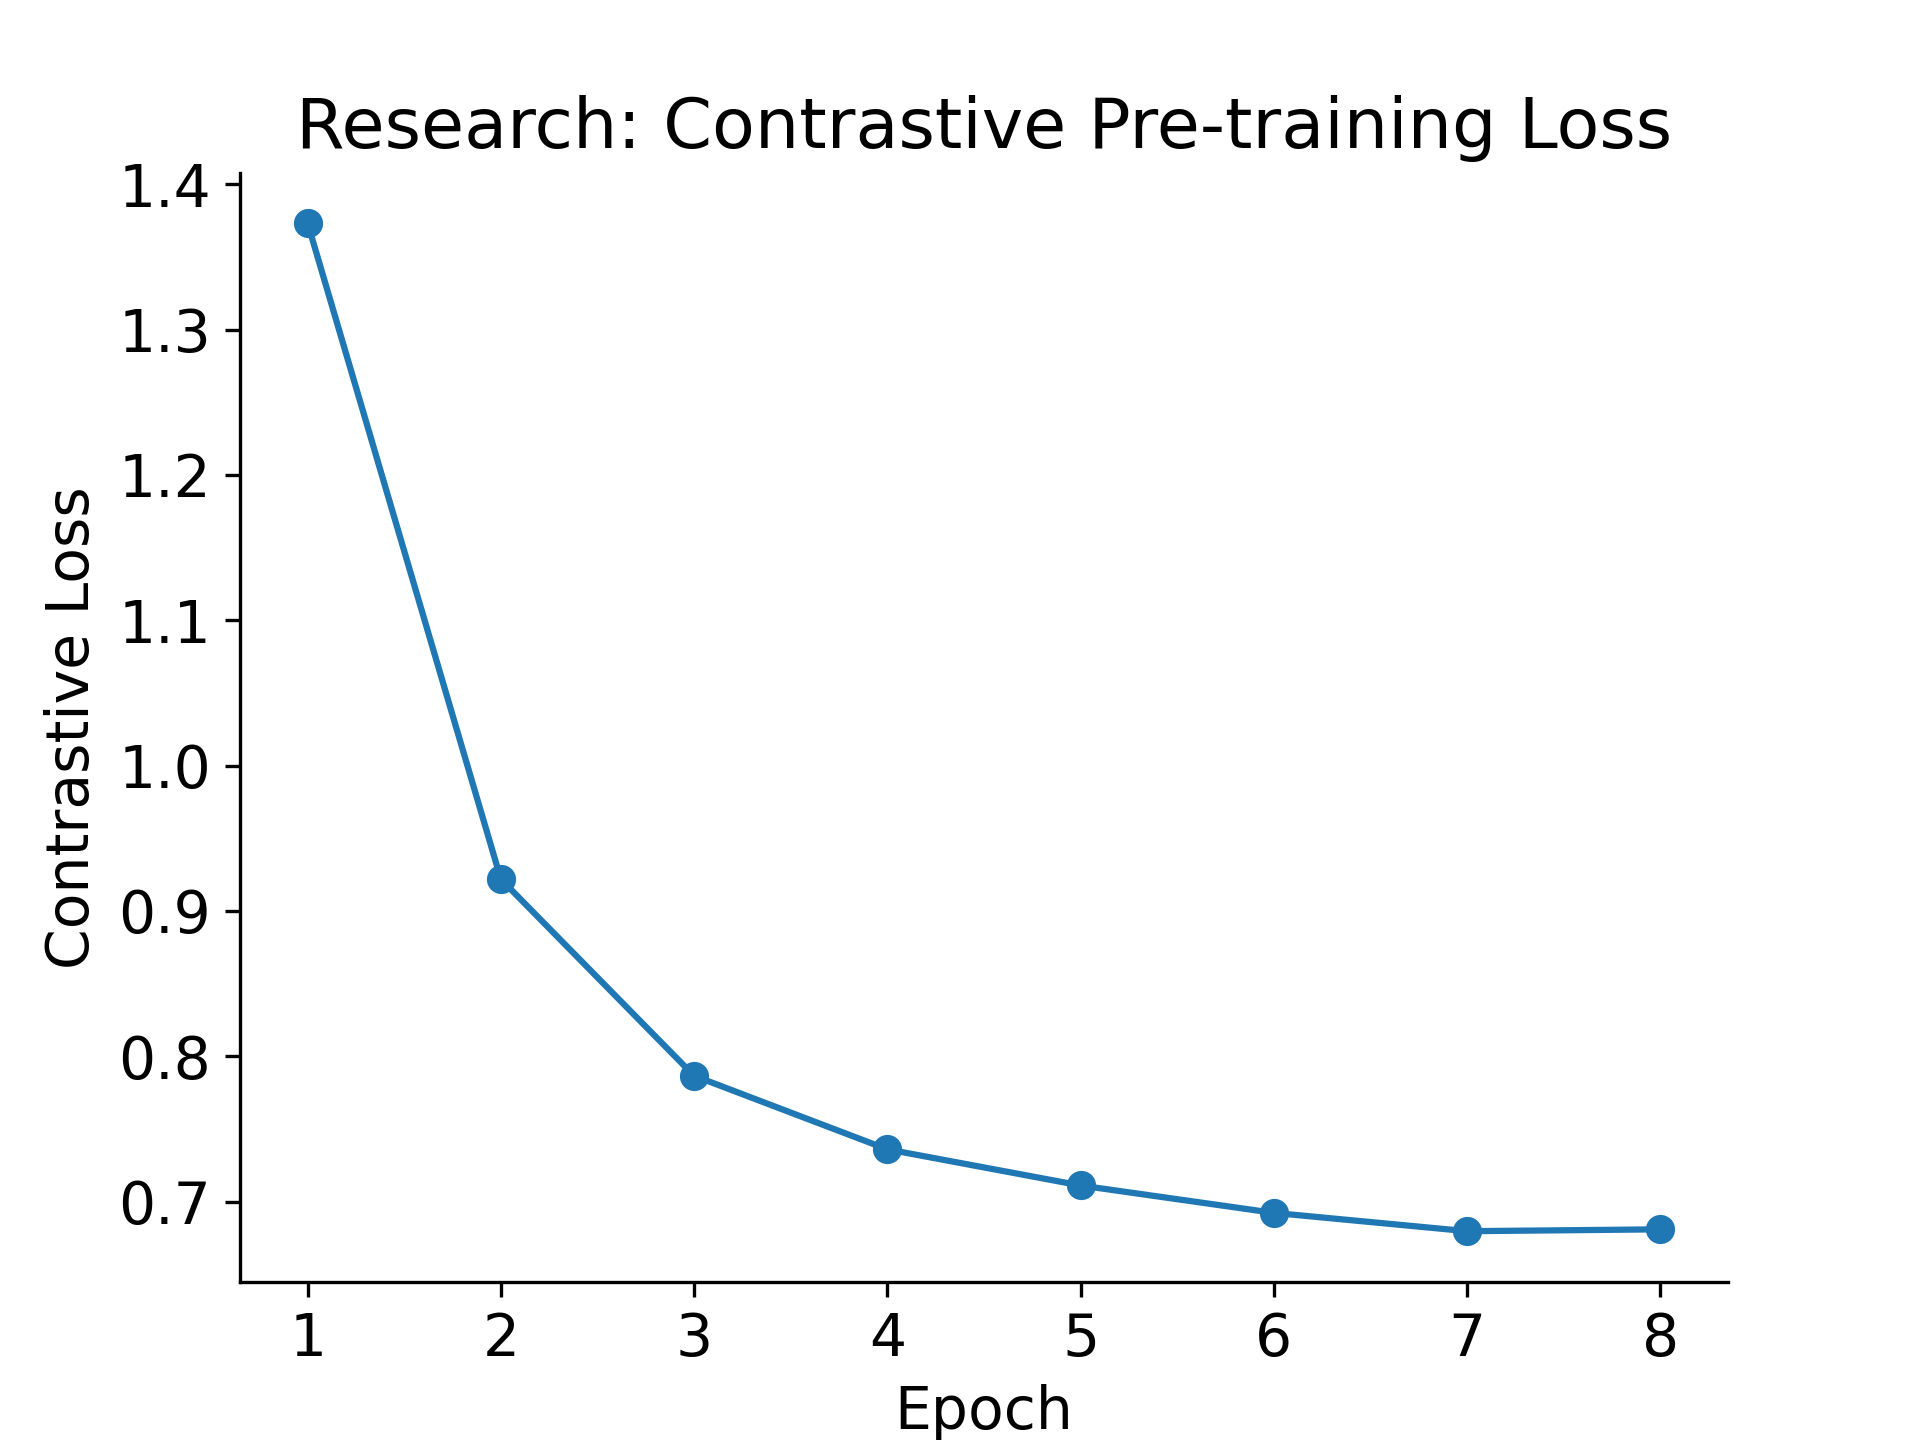
\includegraphics[width=\linewidth]{FIG_Research_Pretrain_Loss.png}
\caption{Contrastive pretraining loss.}
\end{subfigure}
\hfill
\begin{subfigure}{0.49\linewidth}
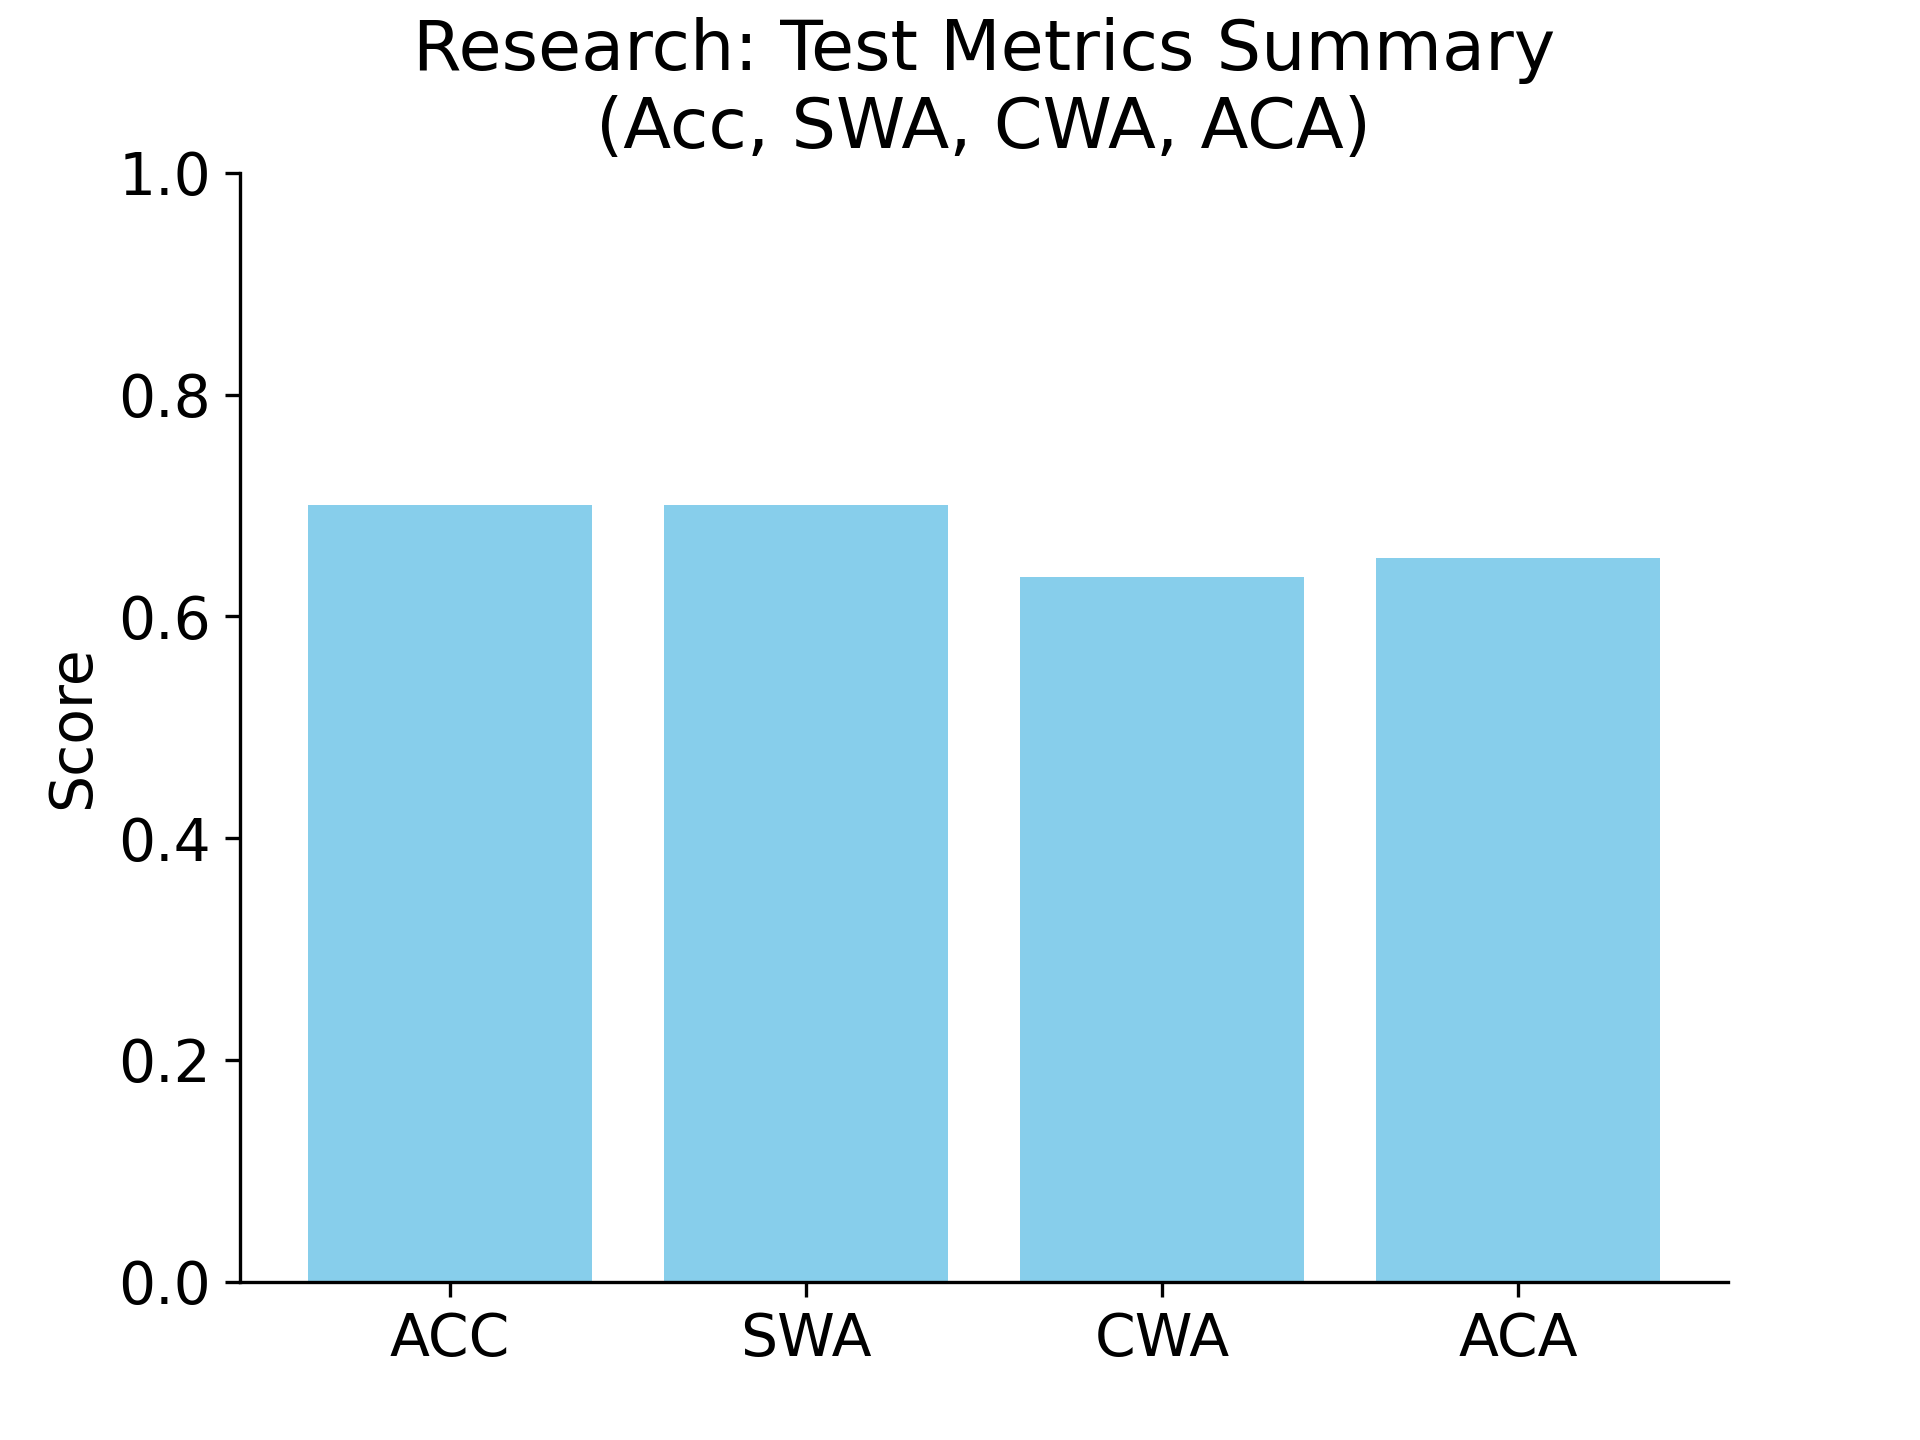
\includegraphics[width=\linewidth]{FIG_Research_Test_Metrics.png}
\caption{Test shape \& color accuracies.}
\end{subfigure}
\caption{Contrastive pretraining yields mildly higher shape accuracy, but color performance drops significantly.}
\label{fig:research}
\end{figure}

Figure~\ref{fig:research} reveals that our best runs showed slight shape gains, though they still exhibited systemic failures in balancing color accuracy. These outcomes highlight the difficulty of improving robustness with standard contrastive approaches.

\section{Conclusion}
While our results offer partial support for the notion that contrastive pretraining can enrich shape-focused features, they also emphasize critical issues with generalization and color misclassification. These pitfalls illustrate how superficial improvements in one metric can mask deeper vulnerabilities in learned representations. Future directions include a more systematic hyperparameter search and a fine-grained analysis of the learned embedding space to mitigate spurious color cues and to ensure success translates to real-world shifts.

\clearpage
% References do not count toward the 4-page limit
\begin{filecontents}{references.bib}
@article{lecun2015deep,
  title={Deep learning},
  author={LeCun, Yann and Bengio, Yoshua and Hinton, Geoffrey},
  journal={Nature},
  volume={521},
  number={7553},
  pages={436--444},
  year={2015},
  publisher={Nature Publishing Group}
}

@inproceedings{chen2020simple,
  title={A simple framework for contrastive learning of visual representations},
  author={Chen, Ting and Kornblith, Simon and Norouzi, Mohammad and Hinton, Geoffrey},
  booktitle={ICML},
  pages={1597--1607},
  year={2020}
}

@article{geirhos2020shortcut,
  title={Shortcut learning in deep neural networks},
  author={Geirhos, Robert and Jacobsen, J{\"o}rn-Henrik and Michaelis, Christian and Zemel, Richard and Brendel, Wieland and Bethge, Matthias and Wichmann, Felix A},
  journal={Nature Machine Intelligence},
  volume={2},
  number={11},
  pages={665--673},
  year={2020},
  publisher={Nature Publishing Group}
}
\end{filecontents}

\bibliographystyle{iclr2025_conference}
\bibliography{references}

\clearpage
\appendix

\section{Supplementary Material}
Here we include additional experimental plots. They provide insight into ablation setups, training dynamics, and validation performance. Some figures illustrate how removing pretraining or employing MLM masking alone affected convergence. Observing them in aggregate reveals the fragility of certain hyperparameter configurations and the recurring theme of color overfitting.

\begin{figure}[h]
\centering
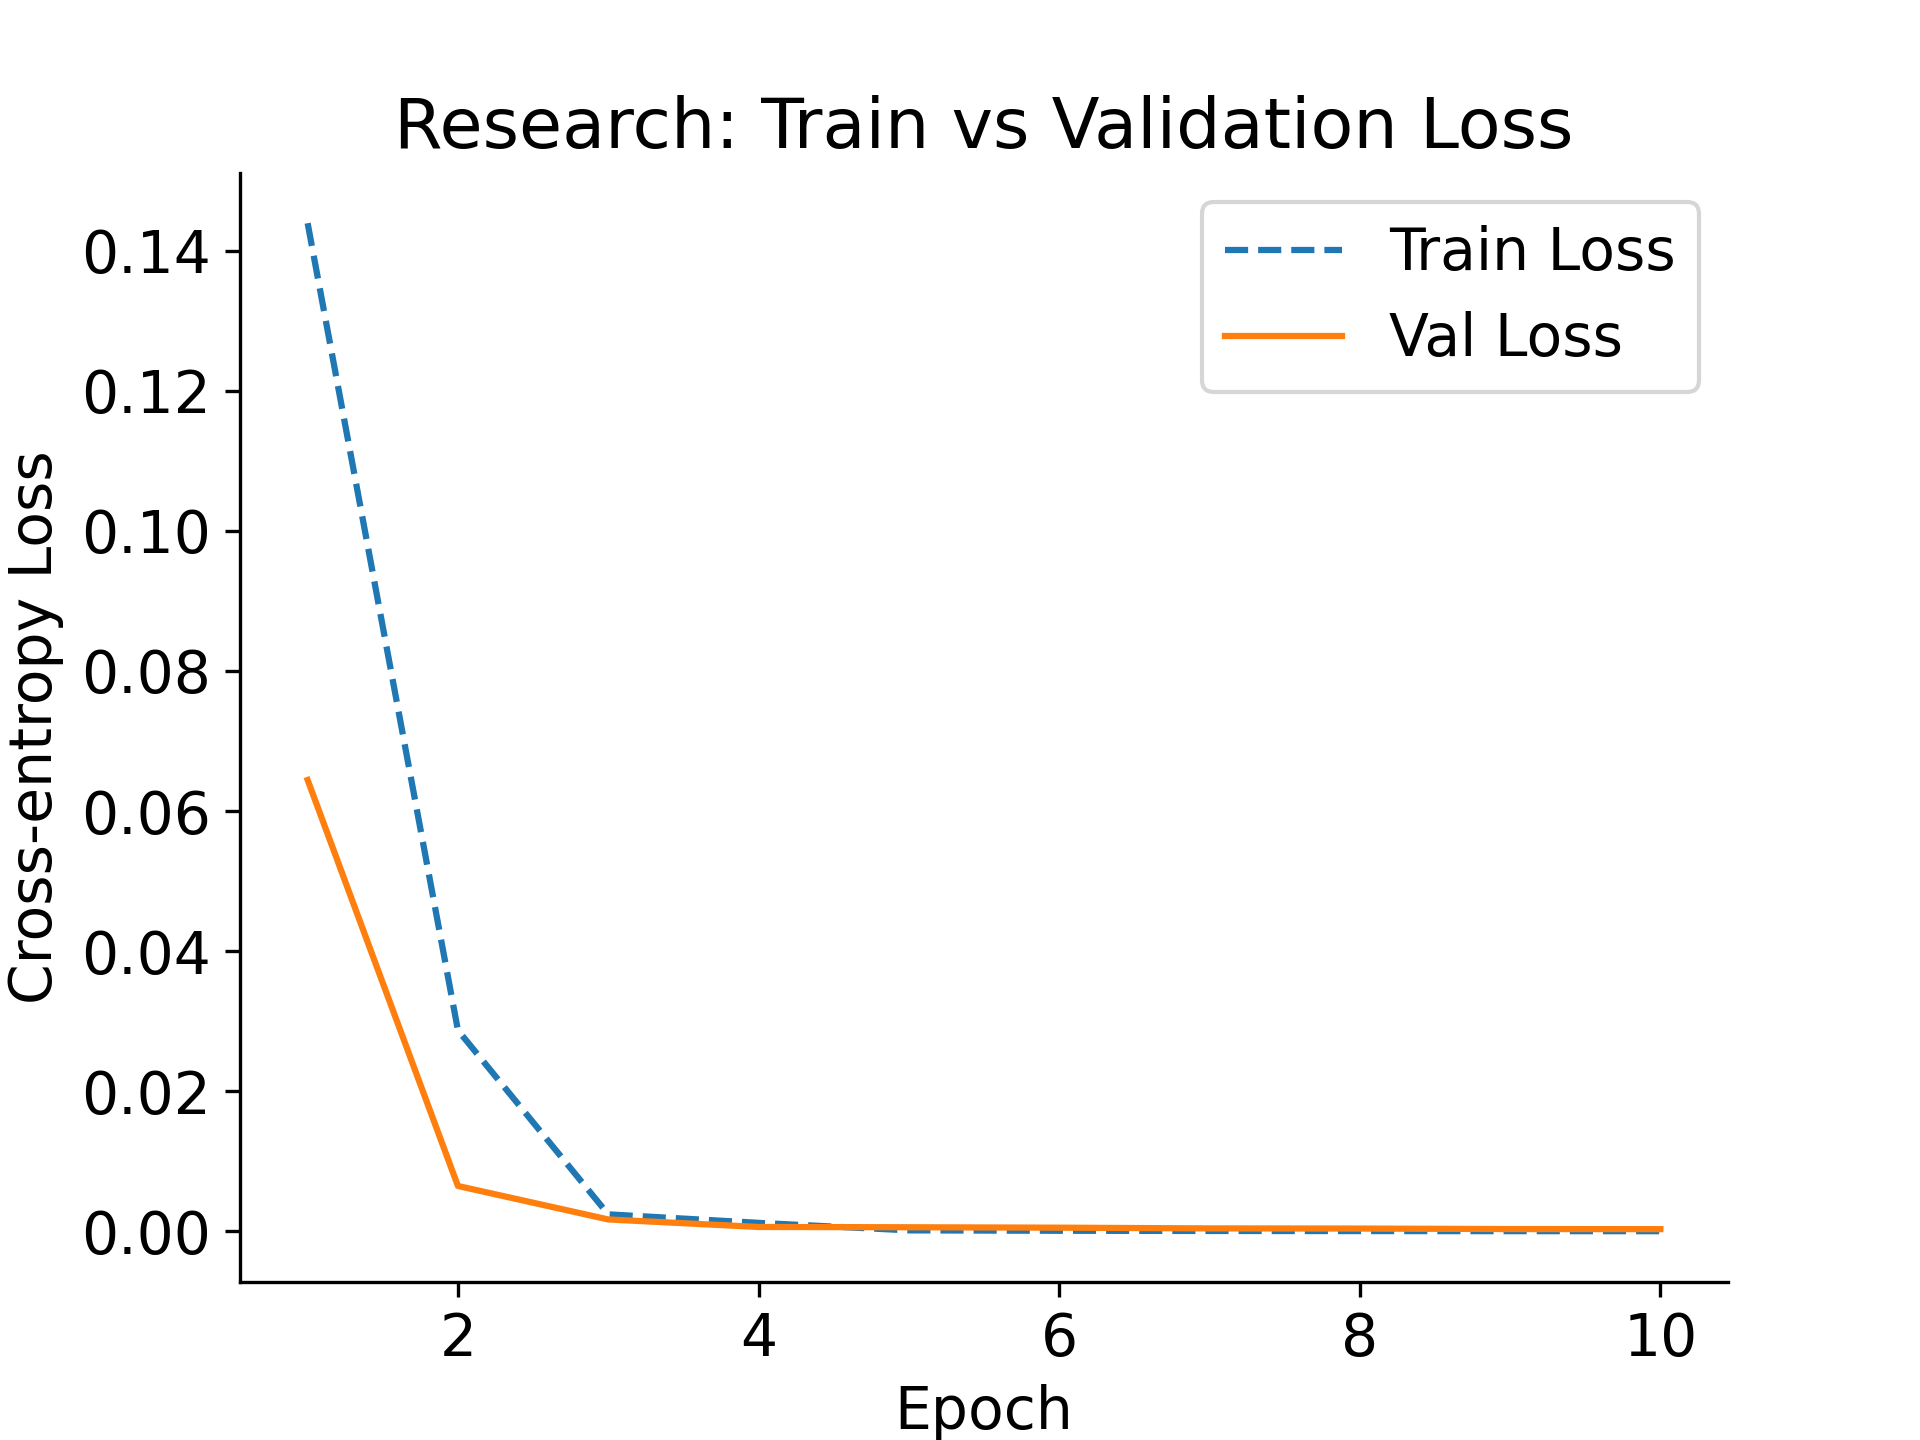
\includegraphics[width=0.49\linewidth]{FIG_Research_Train_Val_Loss.png}
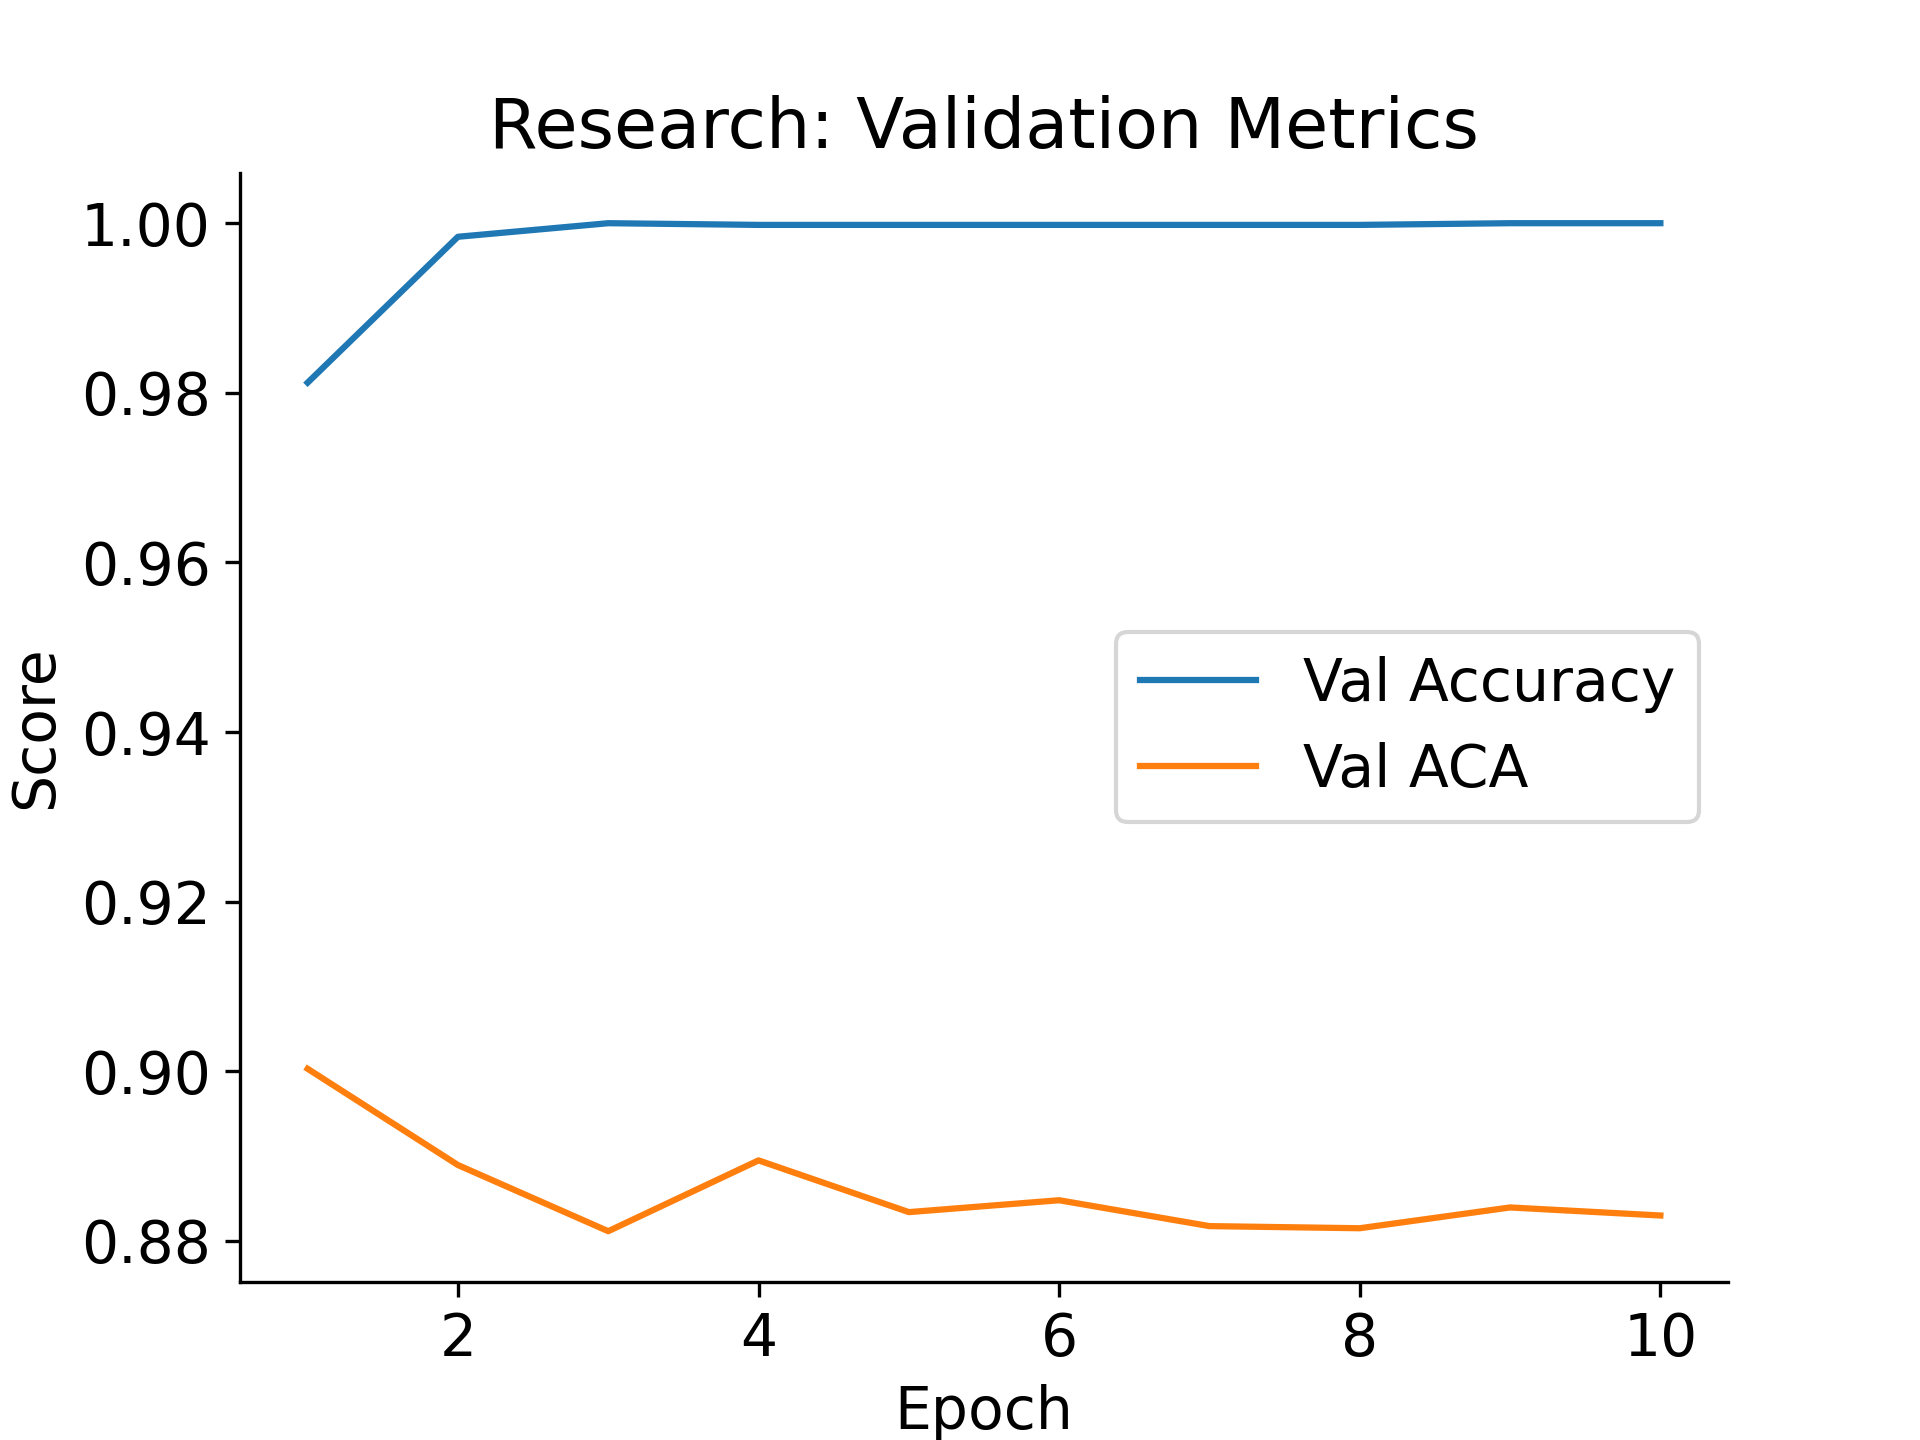
\includegraphics[width=0.49\linewidth]{FIG_Research_Val_Metrics.png}
\caption{Supplementary experiments showing train vs.\ validation loss and validation metrics under various runs.}
\label{fig:supp_research}
\end{figure}

\begin{figure}[h]
\centering
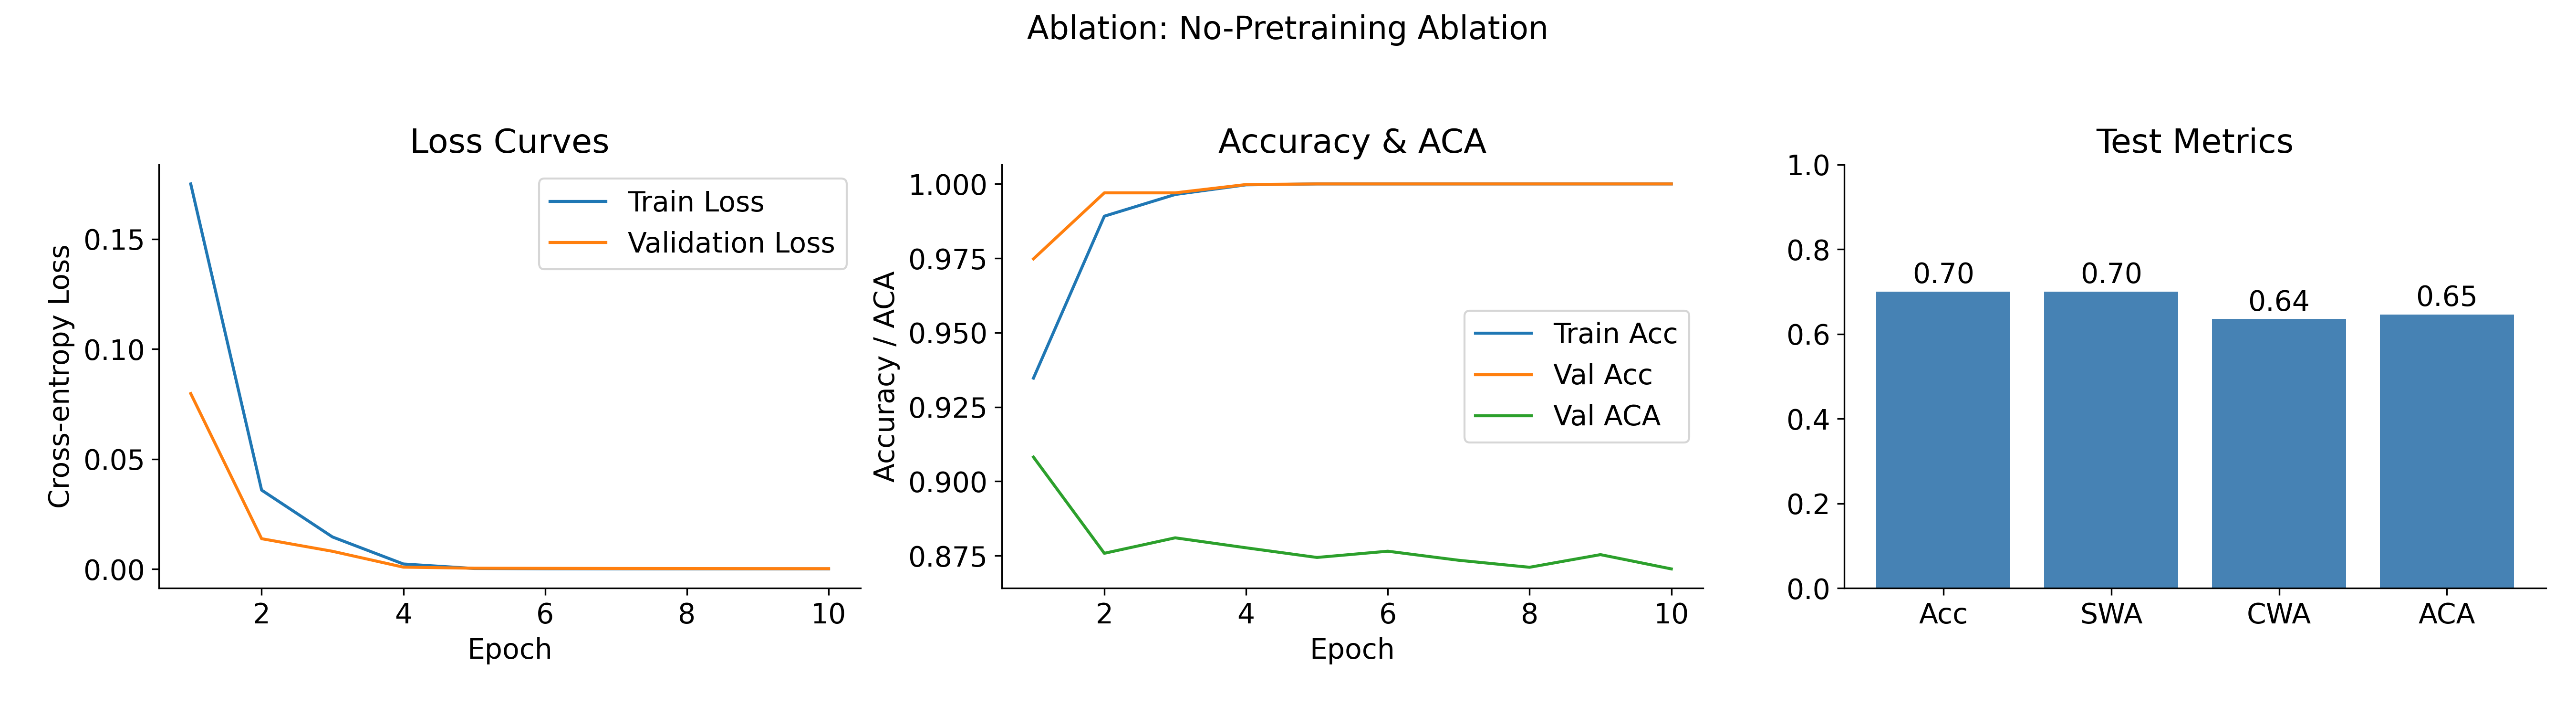
\includegraphics[width=0.49\linewidth]{FIG_Ablation_NoPretraining.png}
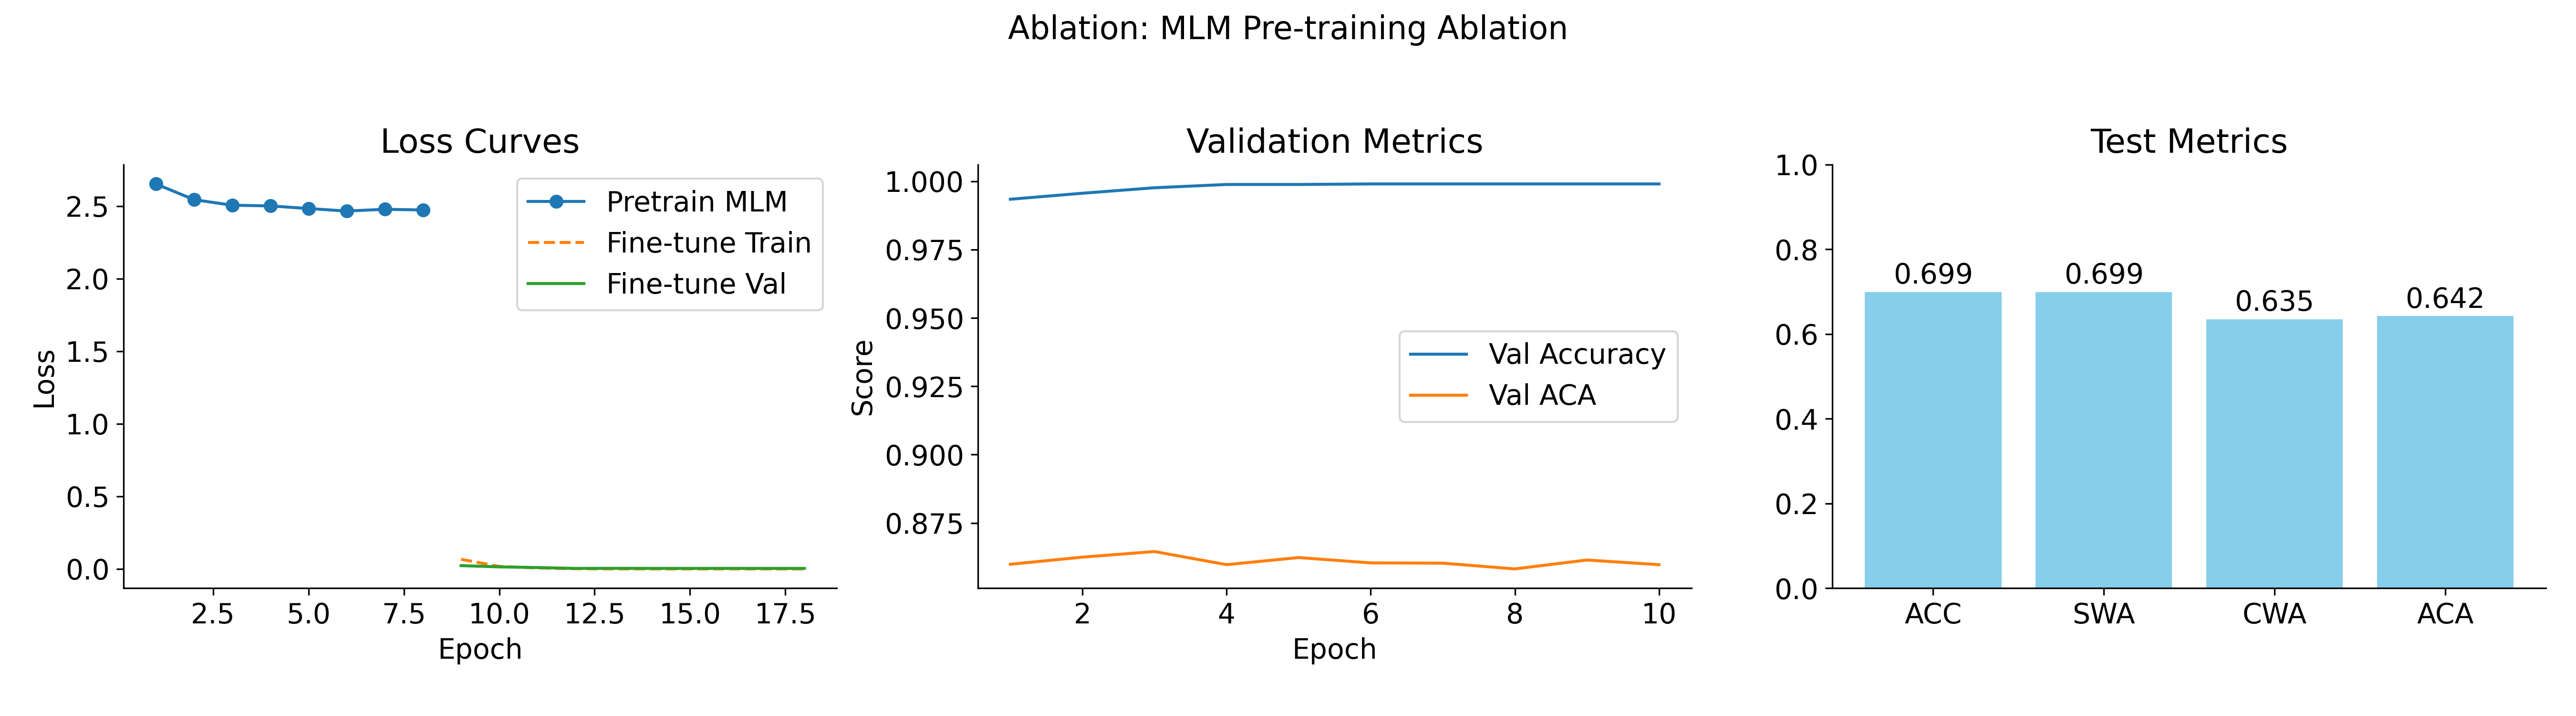
\includegraphics[width=0.49\linewidth]{FIG_Ablation_MLM_Pretrain.png}
\caption{Ablations examining no-pretraining vs.\ MLM-style pretraining.}
\label{fig:ablation}
\end{figure}

\begin{figure}[h]
\centering
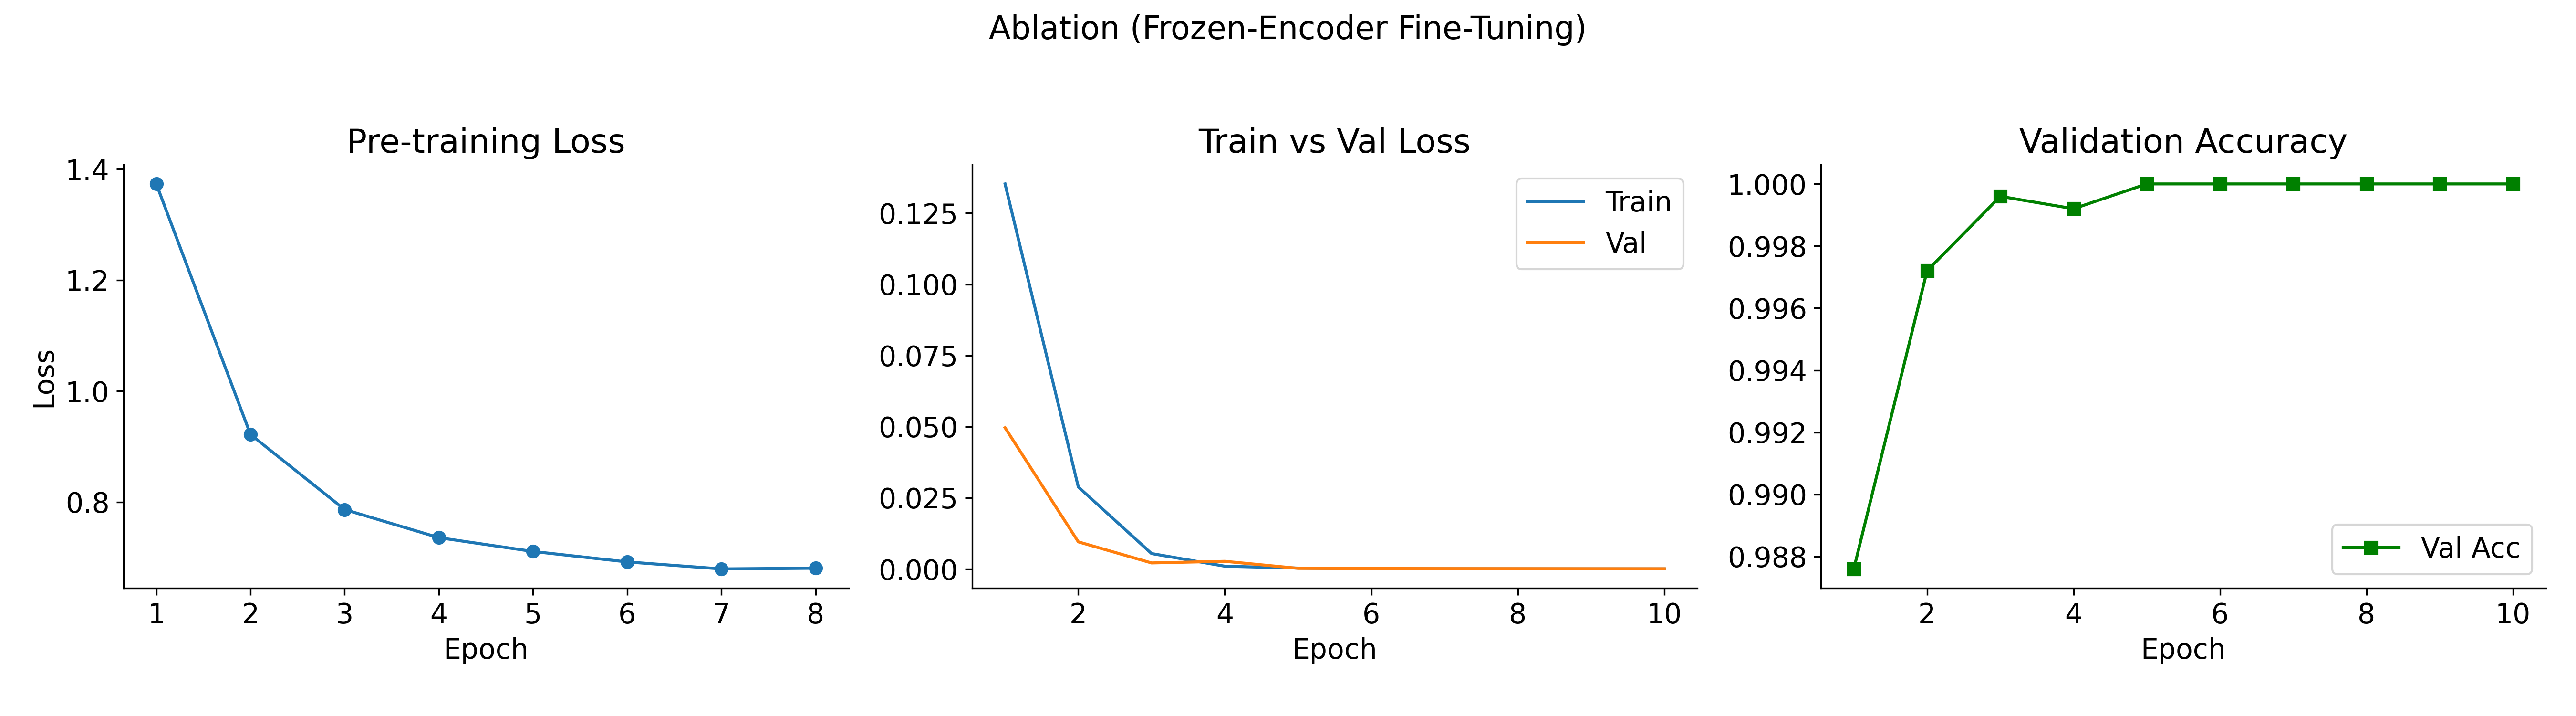
\includegraphics[width=0.49\linewidth]{APP_FrozenEncoder_Ablation.png}
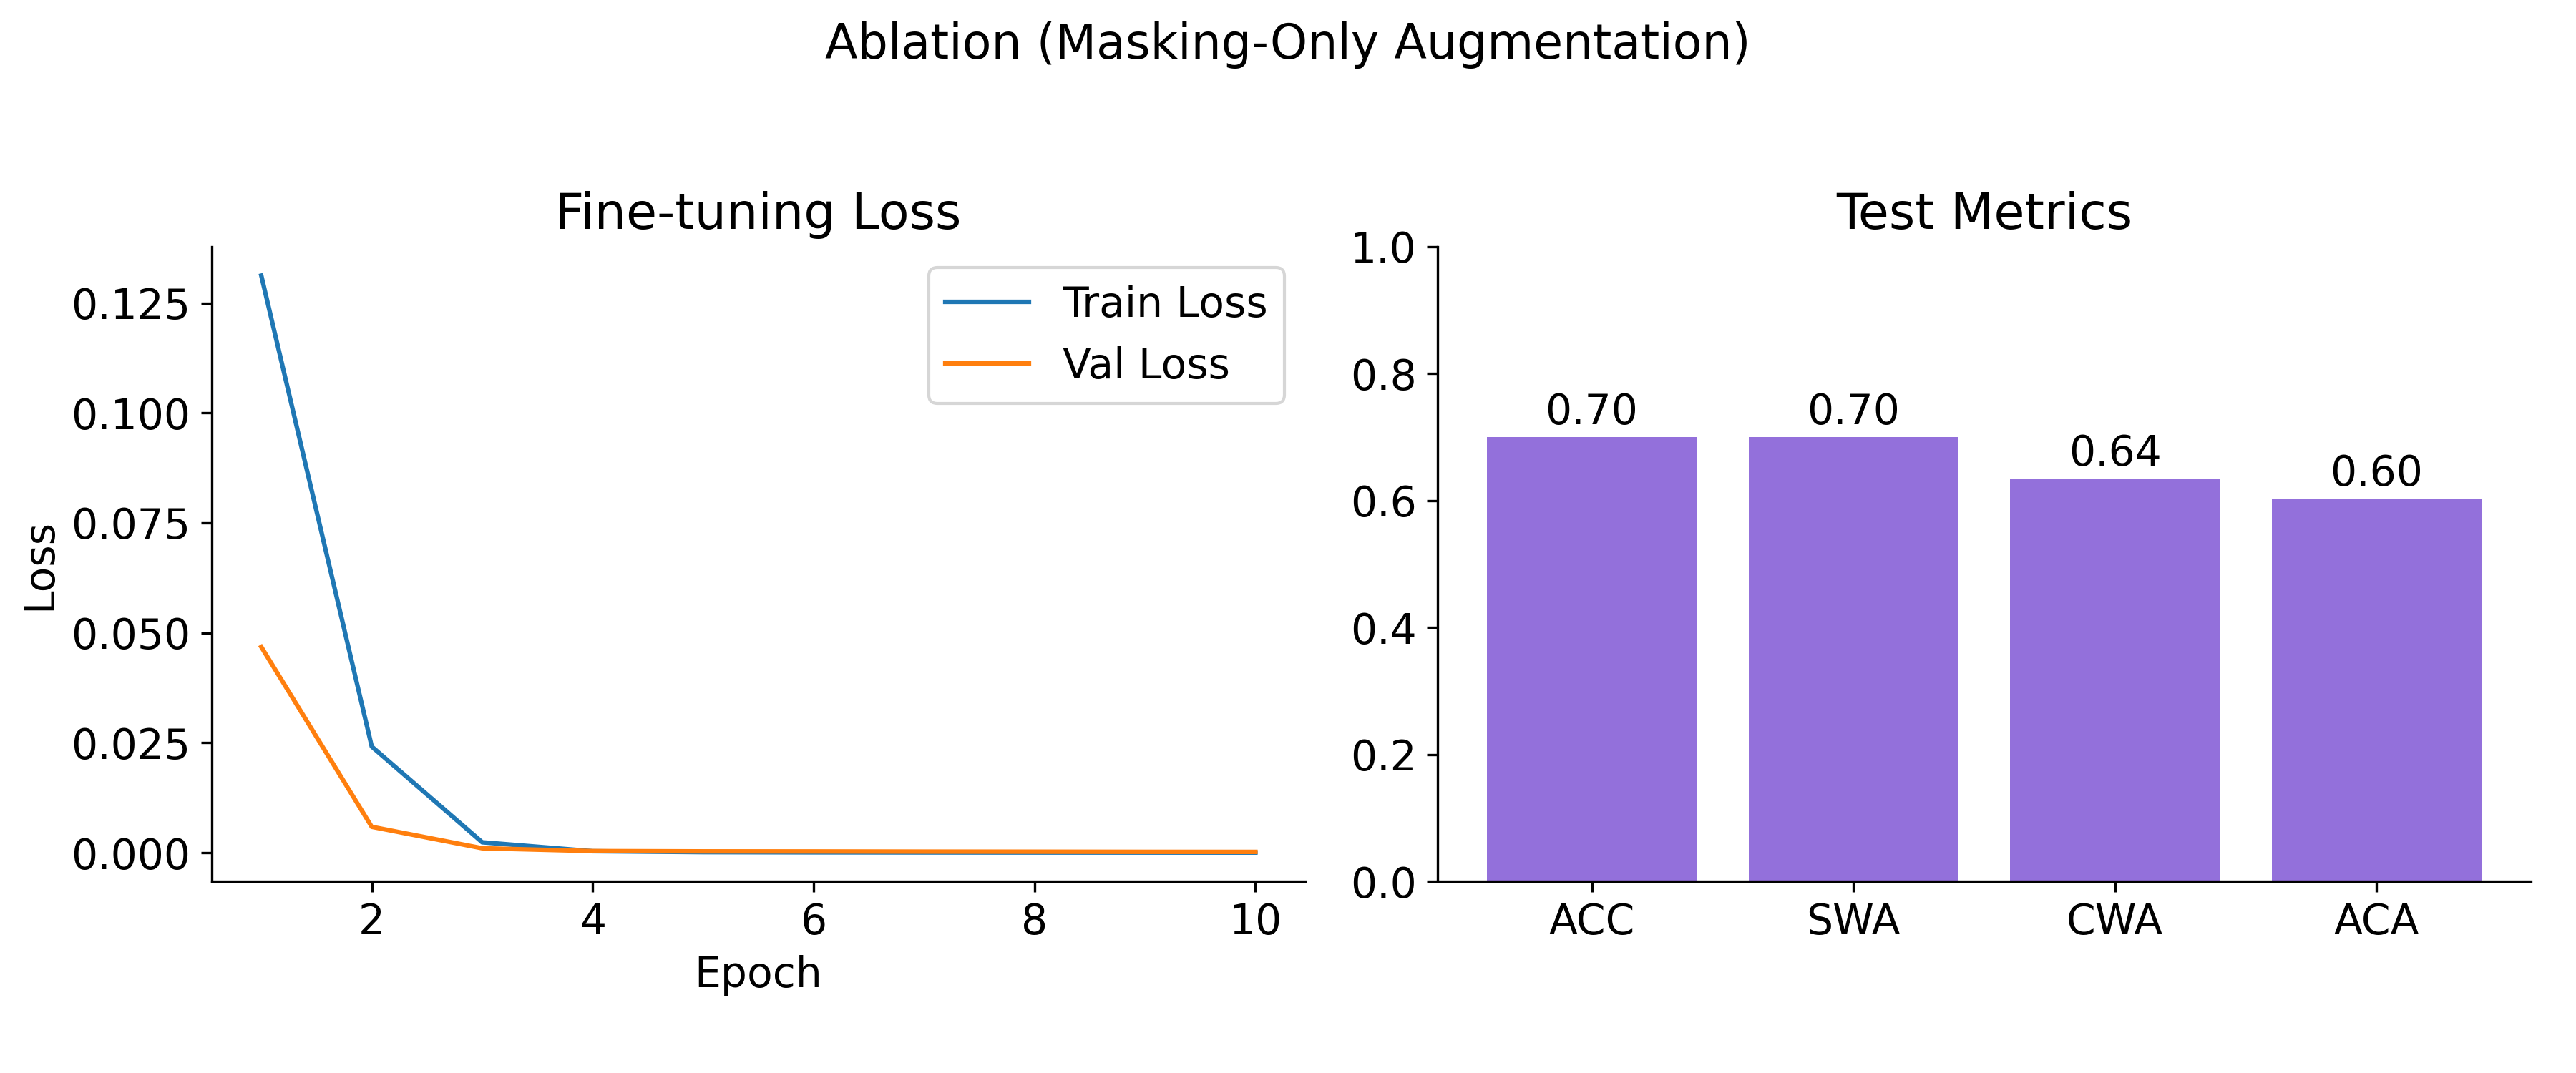
\includegraphics[width=0.49\linewidth]{APP_MaskingOnly_Ablation.png}
\caption{Additional ablations involving frozen encoders and masking-only regimes.}
\label{fig:app_frozen}
\end{figure}

\end{document}